\newprob{1715590598}
{
    % active phys p70 2
    在一個水波槽中,一個直 線脈衝向一個直線障礙物 傳播,如圖。 以下哪一項\textbf{不能}表示反射 脈衝?
    \par{\par\centering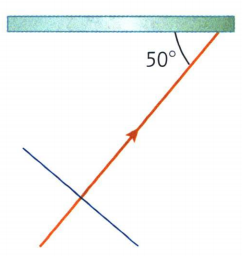
\includegraphics[width=.2\textwidth]{./img/ch2_earlyclass_wave_mc_2024-05-13-20-47-59.png}\par}
    \begin{tasks}(2)
        \task \topalign{\par\centering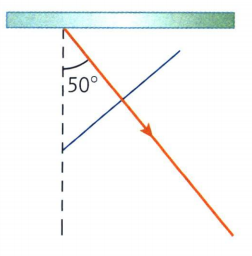
\includegraphics[width=.2\textwidth]{./img/ch2_earlyclass_wave_mc_2024-05-13-20-48-35.png}\par}
        \task \topalign{\par\centering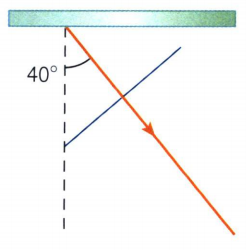
\includegraphics[width=.2\textwidth]{./img/ch2_earlyclass_wave_mc_2024-05-13-20-49-14.png}\par}
        \task \topalign{\par\centering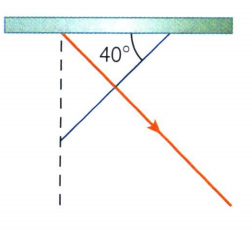
\includegraphics[width=.2\textwidth]{./img/ch2_earlyclass_wave_mc_2024-05-13-20-48-49.png}\par}
        \task \topalign{\par\centering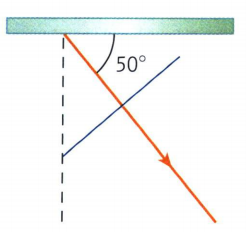
\includegraphics[width=.2\textwidth]{./img/ch2_earlyclass_wave_mc_2024-05-13-20-49-00.png}\par}
    \end{tasks}

}{\mckey A}

\newprob{1715604632}
{
    一條長繩連接至一堵牆壁。一個脈衝沿長繩向牆 壁傳播。長繩上有一顆質點$P$,其$s$-$t$線圖如下 (虛線)。若長繩的張力增加,以下哪一幅圖最能 表示質點$P$新的$s$-$t$ 線圖(以實線表示)?
    \begin{tasks}(2)
        \task \topalign{\par\centering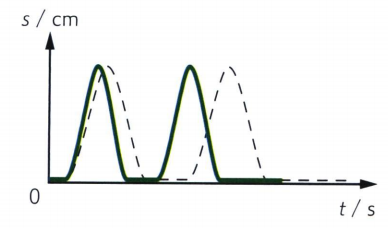
\includegraphics[width=.3\textwidth]{./img/ch2_earlyclass_wave_mc_2024-05-13-20-53-11.png}\par}
        \task \topalign{\par\centering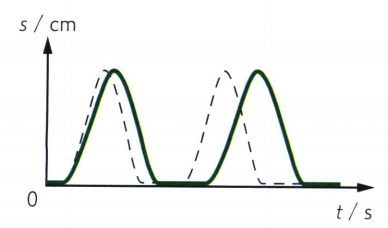
\includegraphics[width=.3\textwidth]{./img/ch2_earlyclass_wave_mc_2024-05-13-20-53-23.png}\par}
        \task \topalign{\par\centering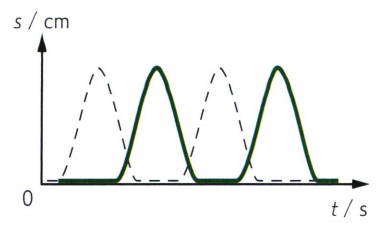
\includegraphics[width=.3\textwidth]{./img/ch2_earlyclass_wave_mc_2024-05-13-20-53-33.png}\par}
        \task \topalign{\par\centering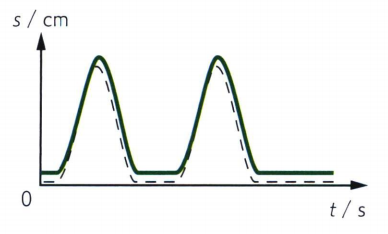
\includegraphics[width=.3\textwidth]{./img/ch2_earlyclass_wave_mc_2024-05-13-20-53-42.png}\par}
    \end{tasks}

}{\mckey A}

\newprob{1715604896}
{
    % active phys p76 q1
    在一個水波槽中,一列 直線水波從深水區進入 淺水區,如圖。 \par 求角$\theta$。
    \par{\par\centering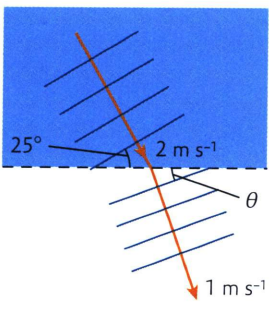
\includegraphics[width=.25\textwidth]{./img/ch2_earlyclass_wave_mc_2024-05-13-20-55-27.png}\par}
    \begin{tasks}
        \task \dg{12.2}
        \task \dg{12.5}
        \task \dg{50.0}
        \task \dg{57.7}
    \end{tasks}
}{\mckey A}

\newprob{1715604988}
{
    % q2
    一列圓形水波原在深 水區傳播,正要進入 淺水區,如圖。 以下哪一幅圖最可能 表示淺水區的波動圖 案?
    \par{\par\centering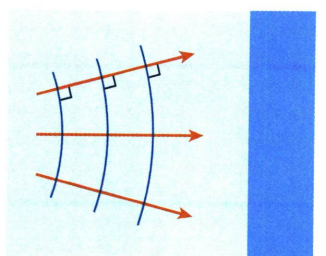
\includegraphics[width=.3\textwidth]{./img/ch2_earlyclass_wave_mc_2024-05-13-20-56-41.png}\par}
    \begin{tasks}(2)
        \task \topalign{\par\centering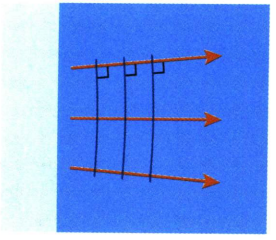
\includegraphics[width=.25\textwidth]{./img/ch2_earlyclass_wave_mc_2024-05-13-20-57-59.png}\par}
        \task \topalign{\par\centering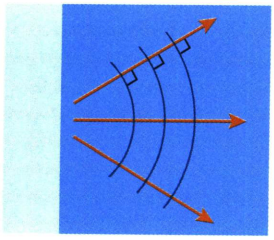
\includegraphics[width=.25\textwidth]{./img/ch2_earlyclass_wave_mc_2024-05-13-20-58-36.png}\par}
        \task \topalign{\par\centering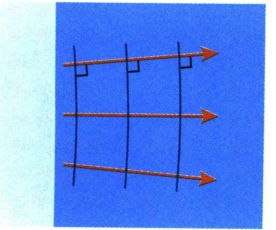
\includegraphics[width=.25\textwidth]{./img/ch2_earlyclass_wave_mc_2024-05-13-20-58-16.png}\par}
        \task \topalign{\par\centering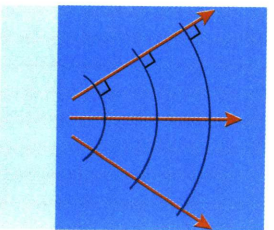
\includegraphics[width=.25\textwidth]{./img/ch2_earlyclass_wave_mc_2024-05-13-20-58-26.png}\par}
    \end{tasks}

}{\mckey A}

\newprob{1715605218}
{
    % q3
    一個直線脈衝 $PQ$ 在區域X內以 \qty{6}{cm.s^{-1}} 傳播。 圖示為該脈衝在時間$t=0$、$t=\qty{1}{s}$和$t=\qty{2}{s}$的 位置。
    \par{\par\centering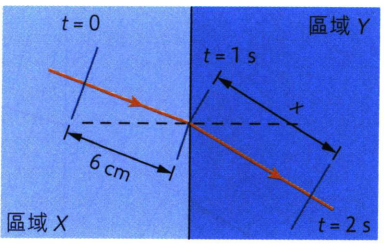
\includegraphics[width=.35\textwidth]{./img/ch2_earlyclass_wave_mc_2024-05-13-21-01-10.png}\par}
    若該脈衝從區域$X$傳播至區域$Y$的折射率為 0.833,求$x$。
    \begin{tasks}
        \task \qty{5}{cm}
        \task \qty{6}{cm}
        \task \qty{7.2}{cm}
        \task 由於入射角和折射角不明,因此不能判斷
    \end{tasks}
}{\mckey C}

\newprob{1715605682}
{
    % active phys p83 q1
    一個點振源S以頻率5 Hz振盪,產生一列波長 為2cm的圓形水波。水波其後通過一道狹縫, 如圖。
    \par{\par\centering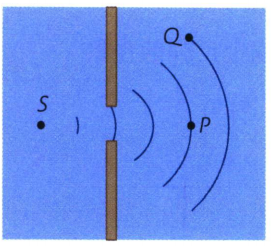
\includegraphics[width=.3\textwidth]{./img/ch2_earlyclass_wave_mc_2024-05-13-21-09-07.png}\par}
    水波從點振源傳播至 P點和Q點的時間分別為 多少?
    \begin{tasks}
        \task [] \textbf{P} \tab\tab \textbf{Q}
        \task \qty{0.5}{s} \tab\tab \qty{0.75}{s}
        \task \qty{0.8}{s} \tab\tab \qty{0.8}{s}
        \task \qty{0.8}{s} \tab\tab \qty{1}{s}
        \task \qty{1}{s} \tab\tab \qty{1.2}{s}
    \end{tasks}

}{\mckey C}

\newprob{1715605925}
{
    % active phys  p86 q1
    在一個水波槽中,一個脈衝向一個障礙物傳播, 如圖。
    \par{\par\centering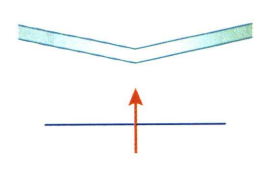
\includegraphics[width=.3\textwidth]{./img/ch2_earlyclass_wave_mc_2024-05-13-21-13-20.png}\par}
    以下哪一幅圖最能表示反射脈衝?
    \begin{tasks}(2)
        \task \topalign{\par\centering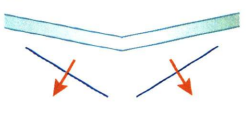
\includegraphics[width=.25\textwidth]{./img/ch2_earlyclass_wave_mc_2024-05-13-21-13-43.png}\par}
        \task \topalign{\par\centering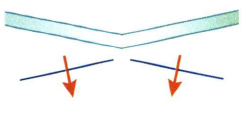
\includegraphics[width=.25\textwidth]{./img/ch2_earlyclass_wave_mc_2024-05-13-21-13-58.png}\par}
        \task \topalign{\par\centering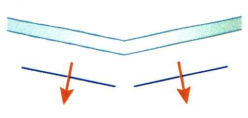
\includegraphics[width=.25\textwidth]{./img/ch2_earlyclass_wave_mc_2024-05-13-21-14-24.png}\par}
        \task \topalign{\par\centering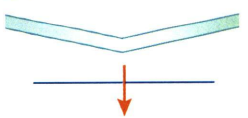
\includegraphics[width=.25\textwidth]{./img/ch2_earlyclass_wave_mc_2024-05-13-21-14-09.png}\par}
    \end{tasks}

}{\mckey A}

\newprob{1715606464}
{
    % q3
    一列直線水波從淺水區向深水區傳播。圖示為深 水區的波動圖形。
    \par{\par\centering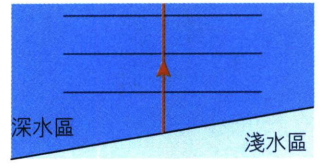
\includegraphics[width=.3\textwidth]{./img/ch2_earlyclass_wave_mc_2024-05-13-21-21-48.png}\par}
    以下哪一幅圖最能表示在淺水區的波動圖形?
    \begin{tasks}(2)
        \task \topalign{\par\centering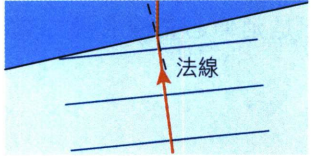
\includegraphics[width=.25\textwidth]{./img/ch2_earlyclass_wave_mc_2024-05-13-21-22-04.png}\par}
        \task \topalign{\par\centering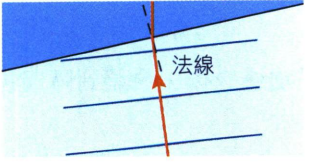
\includegraphics[width=.25\textwidth]{./img/ch2_earlyclass_wave_mc_2024-05-13-21-22-19.png}\par}
        \task \topalign{\par\centering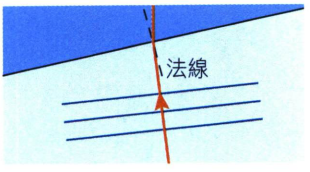
\includegraphics[width=.25\textwidth]{./img/ch2_earlyclass_wave_mc_2024-05-13-21-22-29.png}\par}
        \task \topalign{\par\centering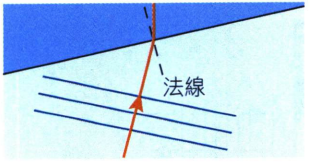
\includegraphics[width=.25\textwidth]{./img/ch2_earlyclass_wave_mc_2024-05-13-21-22-37.png}\par}
    \end{tasks}

}{\mckey C}

\newprob{1715606602}
{
    % q4
    一列直線水波從一個區域 傳播至另一個,如圖。 以下哪一項最能表示兩個 區域之間的邊界?
    \par{\par\centering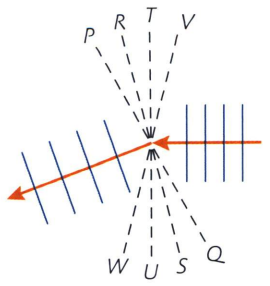
\includegraphics[width=.25\textwidth]{./img/ch2_earlyclass_wave_mc_2024-05-13-21-24-16.png}\par}
    \begin{tasks}
        \task $PQ$
        \task $RS$
        \task $TU$
        \task $VW$
    \end{tasks}
}{\mckey D}

\newprob{1715606686}
{
    % q5
    在一個水波槽中,一根振動的直棒產生一列直線 水波,如圖。
    \par{\par\centering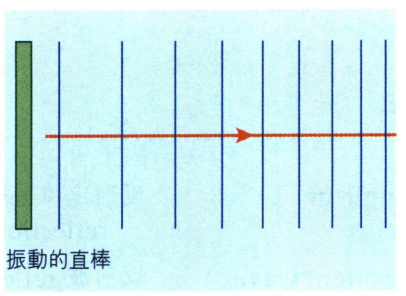
\includegraphics[width=.35\textwidth]{./img/ch2_earlyclass_wave_mc_2024-05-13-21-26-07.png}\par}
    從左至右,波陣面之間越來越密,哪些是可能的 原因?
    \begin{statements}
        \task 水波槽的水深從左至右逐漸減少。
        \task 直棒振動的頻率逐漸下降。
        \task 波傳播時逐漸損失能量。
    \end{statements}
    \begin{tasks}
        \task 只有(1)和(2)
        \task 只有(1)和(3)
        \task 只有(2)和(3)
        \task (1), (2) 和 (3)
    \end{tasks}
}{\mckey A}

\newprob{1715606859}
{
    在一個水波槽中,一列平面水波通過一道縫隙 後,擴散至障礙物後方,如圖。
    \par{\par\centering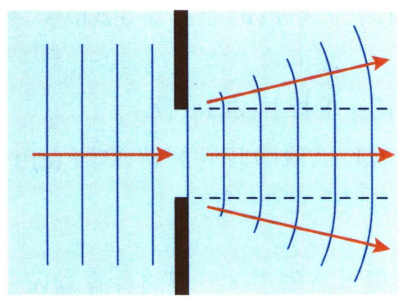
\includegraphics[width=.35\textwidth]{./img/ch2_earlyclass_wave_mc_2024-05-13-21-27-55.png}\par}
    在哪些情況下,水波擴散程度更大?
    \begin{statements}
        \task 水深變深。
        \task 障礙物變厚。
        \task 縫隙變闊。
    \end{statements}
    \begin{tasks}
        \task 只有(1)
        \task 只有(3)
        \task 只有(1)和(2)
        \task 只有(2)和(3)
    \end{tasks}
}{\mckey A}

\newprob{1715606980}
{
    % active phys p91 * q1
    弘基正待在小船上,船身長$\ell$。一列水波經過船 身,如圖。每秒便有 $N$ 個波峯通過小船。
    \par{\par\centering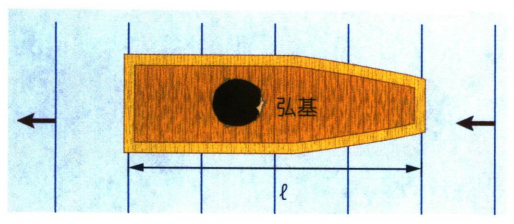
\includegraphics[width=.4\textwidth]{./img/ch2_earlyclass_wave_mc_2024-05-13-21-30-06.png}\par}
    以下哪一項最能表示水波相對弘基的速率?
    \begin{tasks}
        \task $\dfrac{(N-1)\ell}{5}$
        \task $\dfrac{(N-1)\ell}{4}$
        \task $\dfrac{N\ell}{5}$
        \task $\dfrac{N\ell}{4}$
    \end{tasks}

}{\mckey B
    \par{\par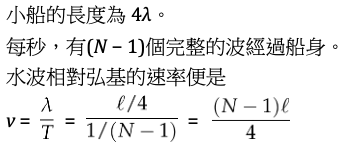
\includegraphics[width=.35\textwidth]{./img/ch2_earlyclass_wave_mc_2024-05-13-21-37-52.png}\par}}

\newprob{1715607083}
{
    在一次地震中,有$S$波(一種地震波)在$E$ 點產 生,並沿綠線所示路徑傳播,如圖所示。已知$S$ 波從地幔向地心傳播時不斷發生折射。$C$點在地 球表面的另一端,而$D$點則在地核和地幔間的界 面上。
    \par{\par\centering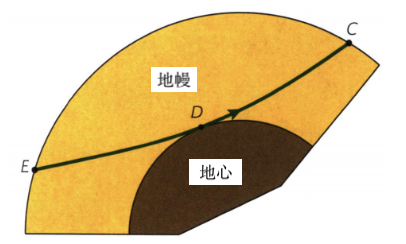
\includegraphics[width=.4\textwidth]{./img/ch2_earlyclass_wave_mc_2024-05-13-21-36-24.png}\par}
    下列哪一項可從上文推斷出來?
    \begin{tasks}
        \task $S$ 波不會展示反射。
        \task $S$波為縱波。
        \task $S$波沿路徑 $ED$ 傳播時不斷加速。
        \task $S$波沿路徑 $EC$ 傳播時,波長逐漸減少。
    \end{tasks}
}{\mckey C
    \par{\par\centering
\includegraphics[width=\textwidth]{./img/ch2_earlyclass_wave_mc_2024-05-13-21-37-32.png}\par}}